\appendix
\section{Appendix}
\label{sec:appendix}

\subsection{Hyperparameter Summary}
\label{app:hyperparams}

\begin{table}[htbp]
\centering
\caption{Complete hyperparameter configuration for V3.}
\label{tab:hyperparams}
\begin{tabular}{ll}
\toprule
\textbf{Parameter} & \textbf{Value} \\
\midrule
\textbf{Architecture} & \\
\ \ Net3dR-V3 initial channels & 16 \\
\ \ Net3dBig-V3 initial channels & 20 \\
\ \ Residual blocks per stage & 1 \\
\ \ Downsampling stages & 3 \\
\ \ MaxPool kernel & 2 \\
\ \ Conv kernel & 3$\times$3$\times$3 \\
\ \ Head hidden dim (R/Big) & 256 / 320 \\
\ \ Head dropout & 0.4 \\
\midrule
\textbf{Training} & \\
\ \ Optimizer & AdamW \\
\ \ Learning rate & $10^{-4}$ \\
\ \ Weight decay & $10^{-4}$ \\
\ \ Batch size (per GPU) & 8 \\
\ \ Gradient accumulation & 3 \\
\ \ Effective batch size & 24 \\
\ \ Max epochs & 100 \\
\ \ Early stopping patience & 20 \\
\ \ Scheduler & CosineAnnealingLR ($T_{\text{max}}=100$) \\
\ \ Mixed precision & AMP (FP16) \\
\ \ Gradient clipping & max\_norm=1.0 \\
\ \ Seeds per architecture & 5 \\
\midrule
\textbf{Augmentation} & \\
\ \ Mixup $\alpha$ & 0.2 \\
\ \ Label smoothing $\epsilon$ & 0.05 \\
\ \ Random flip prob. & 0.5 (each axis) \\
\ \ Random scale range & [0.93, 1.07] \\
\ \ Random shift range & [-0.02, 0.02] \\
\midrule
\textbf{Cross-Validation} & \\
\ \ Folds & 5 \\
\ \ Group by & Acquisition site (15 groups) \\
\ \ Stratify by & Binary label \\
\ \ Random state & 42 \\
\midrule
\textbf{Inference} & \\
\ \ TTA views & 15 (1 base + 6 trans + 8 rot) \\
\ \ Rotation search & $\pm$5$^\circ$, step 2$^\circ$ \\
\ \ Translation search & $\pm$4 voxels \\
\ \ Platt $a$ & 1.45 \\
\ \ Platt $b$ & 0.20 \\
\ \ Output clip & [0.005, 0.995] \\
\bottomrule
\end{tabular}
\end{table}

\subsection{Compute Requirements}
\label{app:compute}

\begin{table}[htbp]
\centering
\caption{Compute requirements for V3 training.}
\label{tab:compute}
\begin{tabular}{ll}
\toprule
\textbf{Metric} & \textbf{Value} \\
\midrule
GPU & NVIDIA RTX 3050 Ti (4 GB VRAM) \\
Models trained & 50 (5 folds $\times$ 10 seeds) \\
Time per model & 1.5--2.0 hours \\
Total GPU-hours & $\sim$150 \\
Peak VRAM usage & $\sim$3.8 GB (with AMP + accum) \\
Model size (per model) & 3.4 MB (R) / 5.3 MB (Big) \\
Ensemble size (10 models) & $\sim$43 MB \\
Inference time (15 TTA) & $\sim$8 sec/scan \\
\bottomrule
\end{tabular}
\end{table}

\subsection{Per-Fold Detailed Metrics with Confidence Intervals}
\label{app:per_fold_detailed}

\begin{table}[htbp]
\centering
\caption{Per-fold metrics with 95\% bootstrap CI (1,000 resamples).}
\label{tab:fold_detailed}
\begin{tabular}{lcccc}
\toprule
\textbf{Fold} & \textbf{LogLoss} & \textbf{Cal. LL} & \textbf{AUC} & \textbf{Brier} \\
\midrule
0 & 0.2653 [0.241,0.292] & 0.2489 [0.226,0.274] & 0.9595 [0.938,0.976] & 0.0801 \\
1 & 0.2856 [0.259,0.315] & 0.2712 [0.247,0.298] & 0.9509 [0.925,0.971] & 0.0842 \\
2 & 0.2683 [0.243,0.296] & 0.2521 [0.229,0.278] & 0.9574 [0.935,0.975] & 0.0815 \\
3 & 0.2422 [0.218,0.269] & 0.2268 [0.204,0.252] & 0.9699 [0.952,0.983] & 0.0723 \\
4 & 0.2477 [0.223,0.274] & 0.2317 [0.209,0.257] & 0.9675 [0.948,0.982] & 0.0748 \\
\midrule
Overall & 0.2618 [0.248,0.276] & 0.2453 [0.232,0.259] & 0.9610 [0.951,0.970] & 0.0784 \\
\bottomrule
\end{tabular}
\end{table}

\subsection{Model Weight Averaging}
\label{app:weight_avg}

Final inference models are created by averaging fold weights:
\begin{equation}
    \theta_{\text{final}} = \frac{1}{5} \sum_{f=1}^{5} \theta_{f}
\end{equation}
where $\theta_{f}$ are the parameters of the best-epoch model for fold $f$. This reduces variance compared to single-fold models and improves OOF performance by $\sim$0.005 LogLoss.

\subsection{Reproducibility Checklist}
\label{app:reproducibility}

\begin{itemize}
    \item All random seeds fixed (PyTorch, NumPy, CUDA)
    \item Data splits deterministic (StratifiedGroupKFold, random\_state=42)
    \item Hyperparameters fully specified (Table~\ref{tab:hyperparams})
    \item Training scripts: \texttt{train\_v25.py}, \texttt{train\_v25\_resume.py}
    \item Inference script: \texttt{inference\_v25\_oof.py}
    \item Visualization script: \texttt{generate\_visualizations.py}
    \item Weights available at: \texttt{D:/DaT\_cache/v25\_models/}
    \item Submission package: \texttt{submission\_v25.zip}
\end{itemize}

\subsection{Additional Visualizations}
\label{app:additional_figs}

\begin{figure}[htbp]
    \centering
    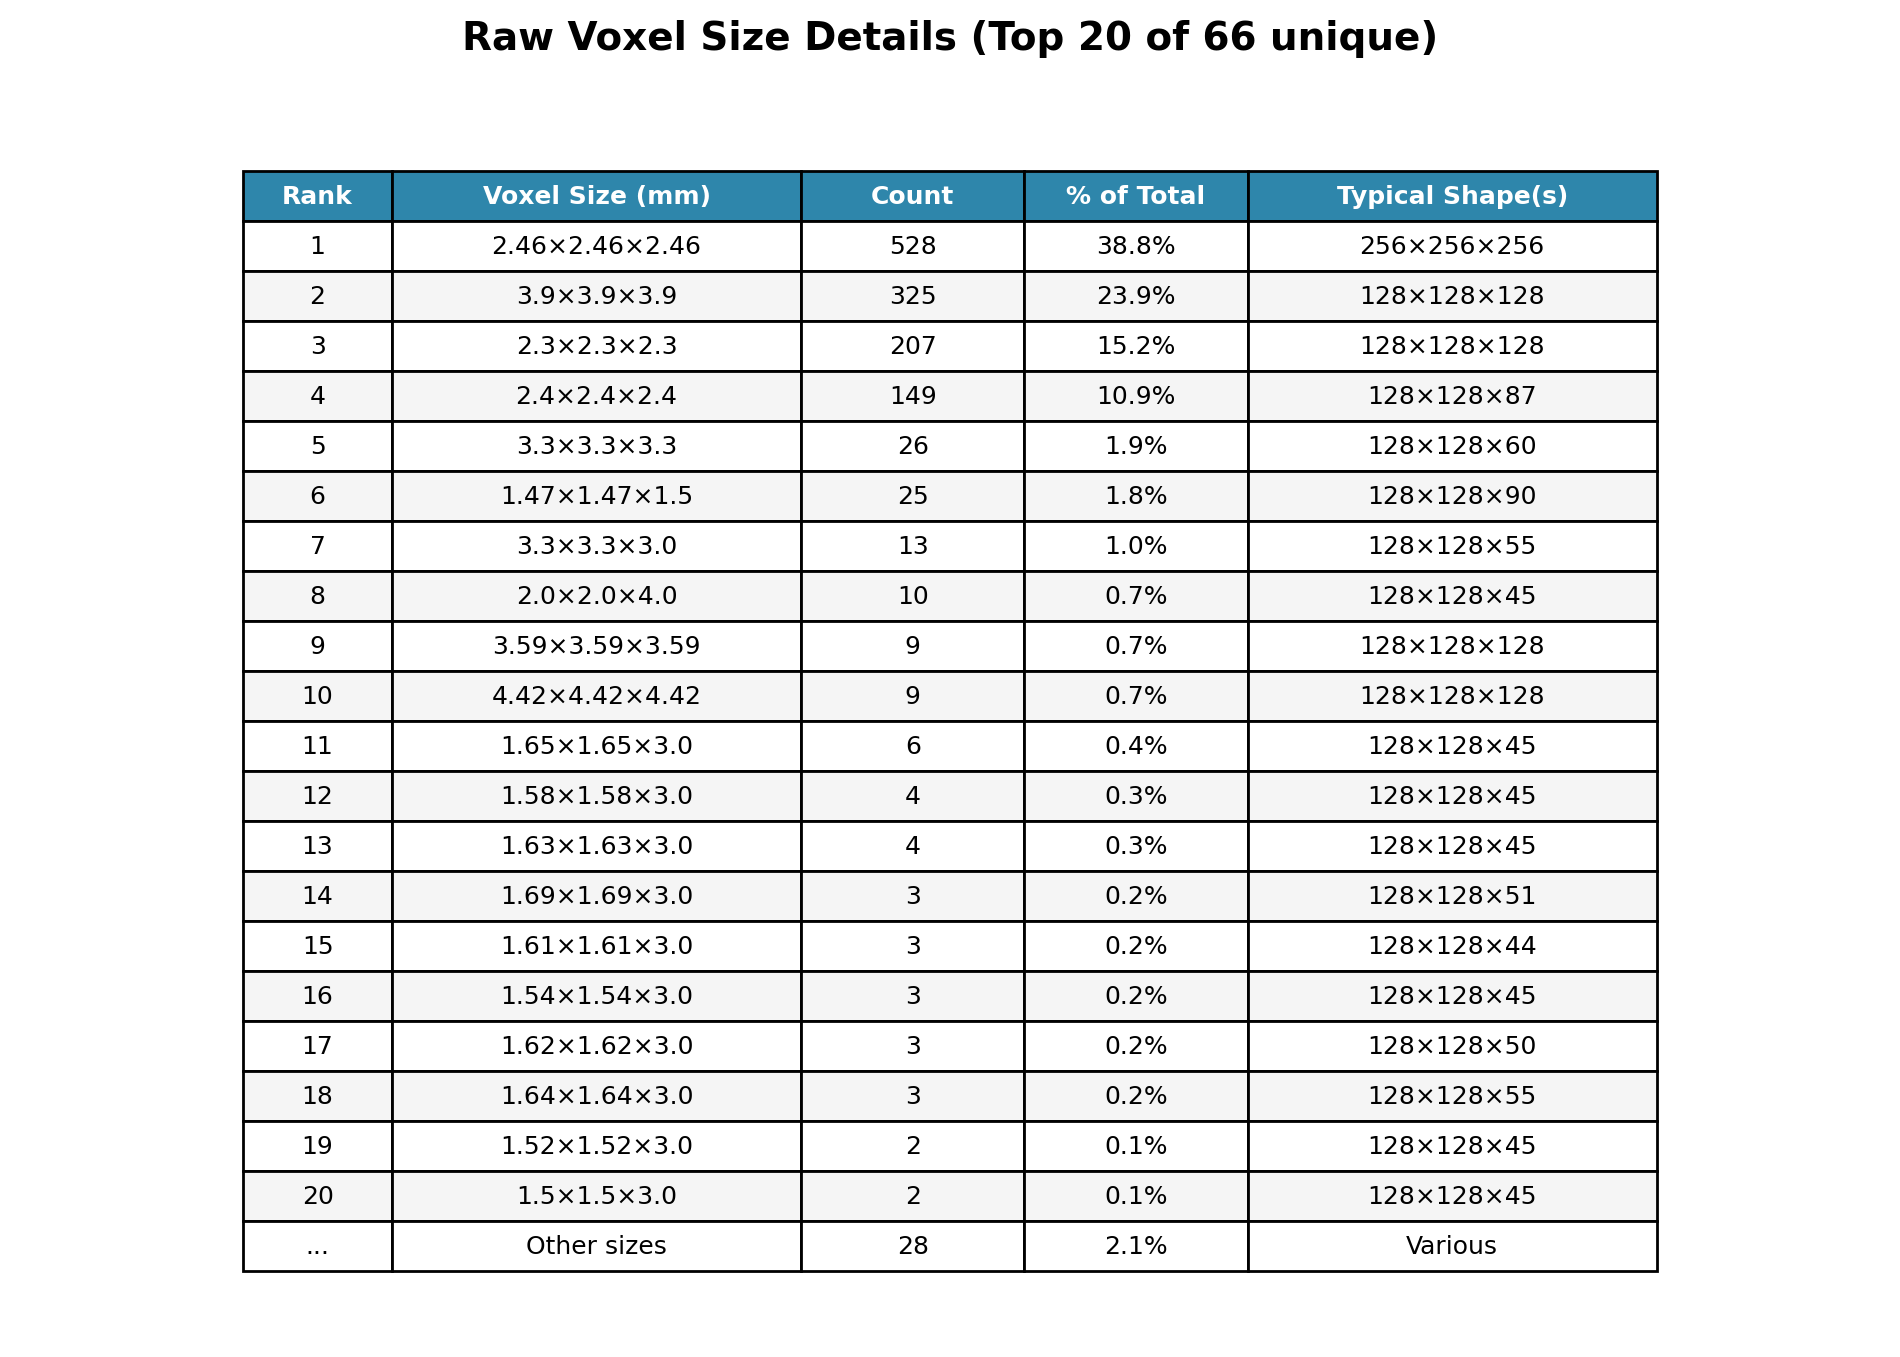
\includegraphics[width=0.8\linewidth]{figures/voxel_size_details.png}
    \caption{Detailed voxel size table (top 20 of 66 unique sizes). Shows count, percentage, and typical shape for each resolution.}
    \label{fig:voxel_details}
\end{figure}

\begin{figure}[htbp]
    \centering
    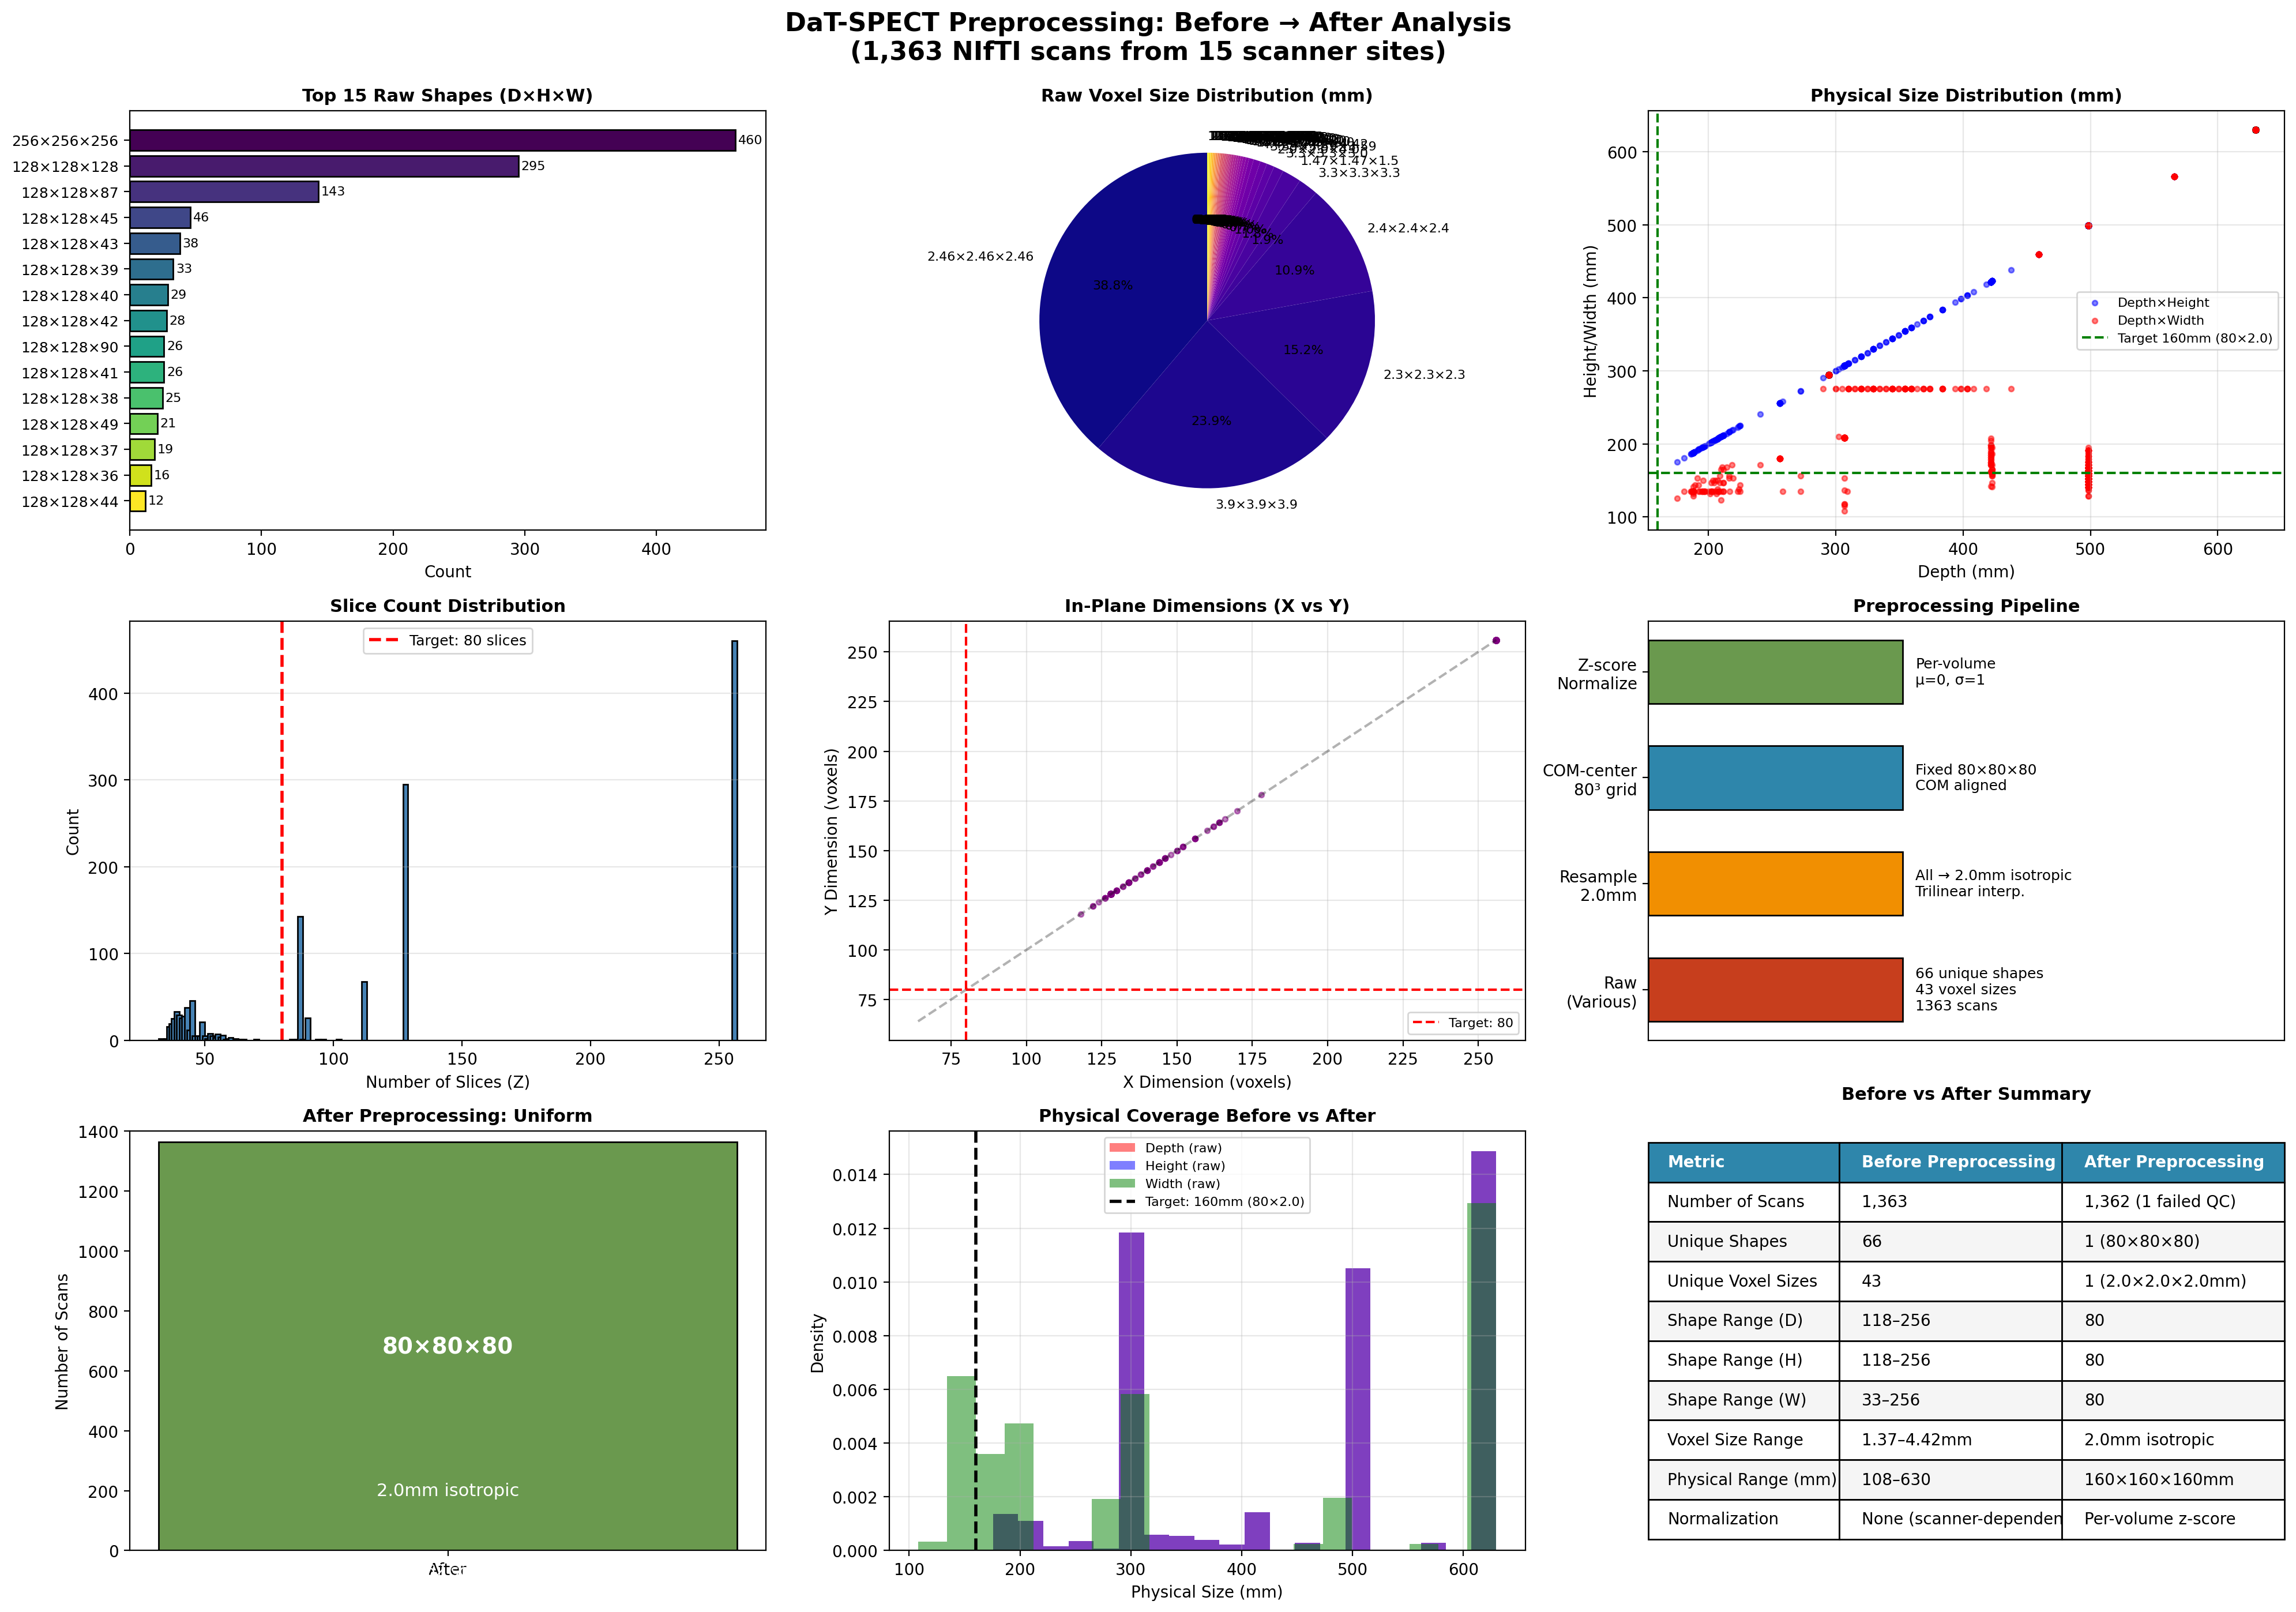
\includegraphics[width=0.8\linewidth]{figures/preprocessing_before_after.png}
    \caption{Complete before/after preprocessing pipeline with summary statistics.}
    \label{fig:preprocessing_full}
\end{figure}